\chapter{Key Concepts and Architecture}

In this section we will go through the architecture of HQL and describe how we
modelled the various of financial instruments in Haskell. We shall introduce
the necessary mathematical finance and conventions as we go along.

\section{Language features}

Functional languages lend themselves well to the domain of finance due
to several reasons such as modularity\cite{hughes:matters-cj} and 
laziness\cite{composingcontracts}. Moreover, the mathematical nature
of finance makes functional languages suitable for valuation due its
inherent mathematical foundation and purity. Haskell's compositionality
promotes code re-use and allows us to easily create new functions from
existing ones. Haskell's standard library features a wide array of
functions for list manipulation which are convenient as this data structure
is used to represent cashflows.\\

Haskell's advanced type system eliminates a whole class of bugs related to 
type errors and its 
class system allows us to define type-safe interfaces for operations on 
financial products who themselves can be represented by Haskell data types. 
Statically typed languages have the advantage of discovering a multitude of
errors at compile time, and the type class system enables us to overload 
functionality in our programs based on our types. This is a very desirable
feature, as we want our financial products to have the same API (e.g. a function 
called \texttt{presentValue} should return the present value regardless of the
product type).\\

Figure \ref{fig:overview} shows an overview of the entities we are dealing with
and situations we wish to model. Ultimately, each item in this figure must somehow
be represented in Haskell using a class or type depending on the the item. We
want to model a library that features financial products, mathematical models
for valutation and finally what we call a pricing engine, which combines the 
these contracts and mathematical models with the current state of the world
in order to produce meaningful measurements of said contract.\\

\begin{figure}[h!]
\begin{center}
\begin{minipage}{\linewidth}
\makebox[\linewidth]{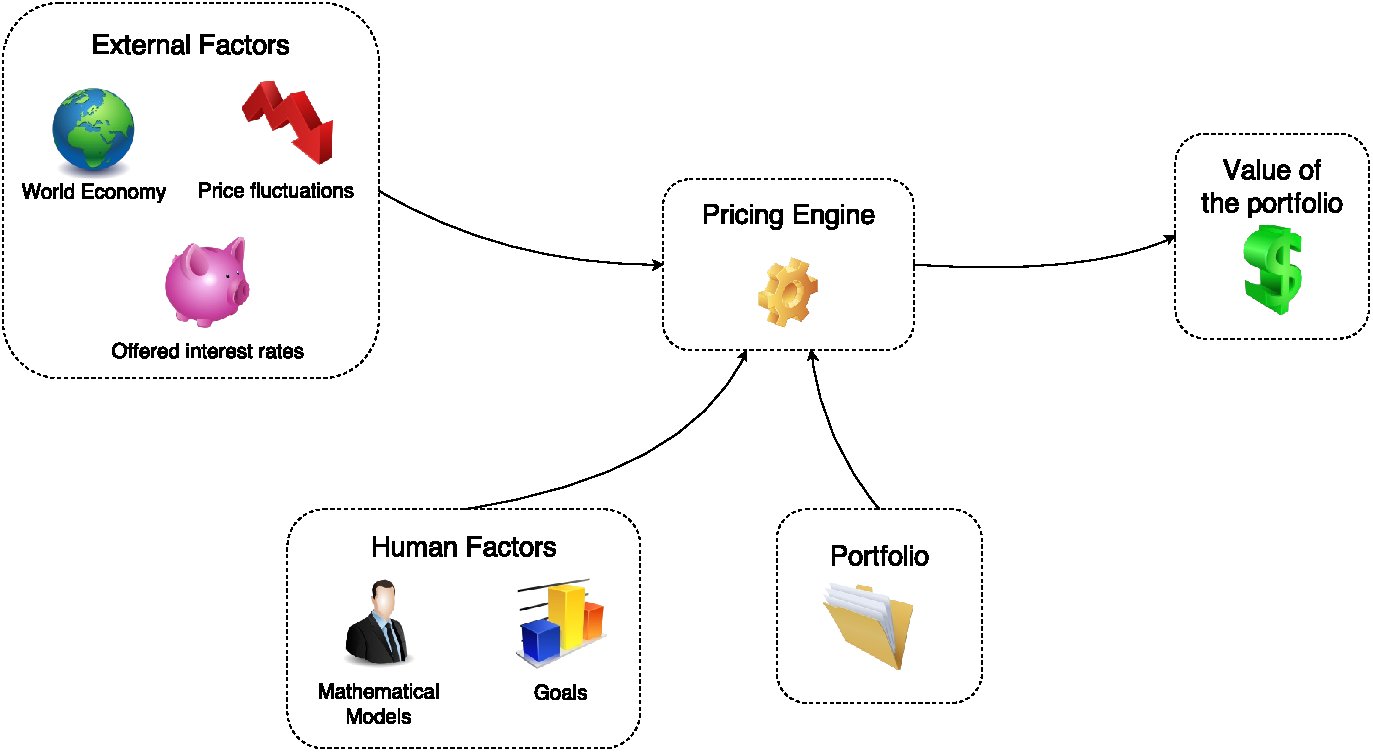
\includegraphics[keepaspectratio=true,scale=0.6]{images/Overview.pdf}}
\caption{Overview of what we want to model.}
\label{fig:overview}
\end{minipage}
\end{center}
\end{figure}

We shall begin with the modelling aspects and provide the reader with the
matematical background required. Thereafter we will present the contracts, and
finally how such a pricing engine is modelled. 

\section{Interest Rates}

We begin our introduction to mathematical finance with a concept familiar to
most, namely interest rates, which specify the amount of return on
investing an amount of money for a set amount of time. This can be formulated
using a very simple equation, which we will demonstrate with a one year flat
interest rate on a deposits account:

\begin{equation}\label{eq:lincomp}
FV_T = N (1 + R_T)
\end{equation}

where $FV_T$ denotes the future value in $T=1$ periods, $N$ is the principal
and $R_T$ is the rate over the period $T$\footnote{$T$ is also referred to as the
\emph{tenor}.}. Extending this to multiple years we introduce the 
concept of compound interest, which is simply the formula above reapplied
a number of times. The intuitive approach is
that the compound interest is the return from reinvesting previously invested
capital. Mathematically, this return can be formulated as an exponentially 
compounded interest rate:

\begin{equation}\label{eq:expcomp}
FV_{T_n} = N (1 + R_{T_n})^n
\end{equation}

where $FV$ is now dependent on the number of times it is compounded, and is 
therefore also called periodic compounding.
While this model is easy to understand, the world of finance demands much more 
intricate details to correctly interpret it. First, it assumes 
discrete time periods, but we have not specified if this $n$ stands for days, 
months, or years, or what the tenor is. Further, it assumes that compounding
occurs at every period, which is not necessarily so. Equation \ref{eq:expcomp2}
shows how the compounding frequency $m$ (number of times interest is compounded
per year) affects exponential compounding. For instance if $n=1$ and $m=2$ the
equation describes the return on a one-year investment with semiannual compounding.

\begin{equation}\label{eq:expcomp2}
FV_{T_n}^{n,m} = N (1 + \frac{R_{T_n}}{m})^{mn}
\end{equation}

All of these intricacies are critical for correctness of \hql and must
be accounted for in the implementation.\\

Up until this point we have assumed that the compounding is performed at 
discrete intervals. However, as \ref{eq:expcomp} is simply a formula, we may apply 
methods  from calculus to achieve what is known as the continuously compounded interest 
rate. It is defined as the resulting interest rate when we take the limit of 
equation \ref{eq:expcomp} as $m$ goes to infinity:

\begin{equation}
\text{lim}_{n \rightarrow \infty}\; FV_T^n \; = \text{lim}_{n \rightarrow \infty}\; N (1 + R_T)^n
= N e^{RT}
\end{equation}

where $R$ is the continuously compounded interest rate\cite{HULL}. This rate
is much easier to work with in advanced fixed income modelling\cite{cmunk}, 
as we can disregard the details concerning periods and compounding intervals.
Further, it yields sufficiently close numerical results.

\begin{figure}[!htb]
\centering
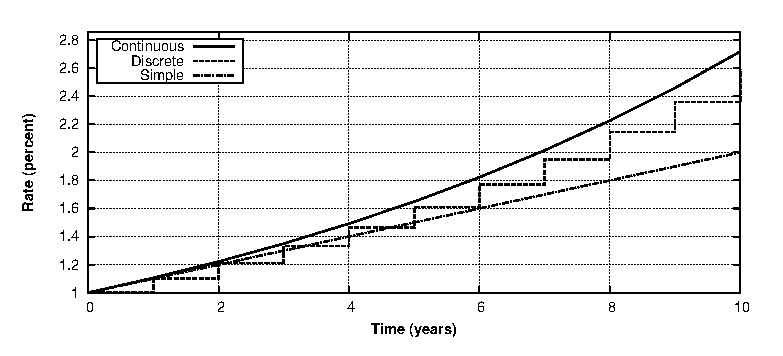
\includegraphics[scale=1.2]{images/comp02.eps}
\caption{How compounding methods influence returns.}
\label{fig:comp02}
\end{figure}

Figure \ref{fig:comp02} shows the influence in rate as a result of the different
kinds of compounding. Note that the return of the different compounding methods
differs after the first year. Furthermore, table \ref{tab:cmptable} gives an 
overview of the relation between compounding functions and time steps.
Periodic compounding is exactly the scenario we modelled in equations 
\ref{eq:expcomp} and \ref{eq:expcomp2}, and the flat rate is described by equation
\ref{eq:lincomp} ("flat" referring to the fact that return scale linearly with
the time that the capital is invested). It should be evident to the reader
that the notion of linear continuously compounded interest rate is absurd,
as we derive it from equation \ref{eq:expcomp}.

\begin{center}  
\begin{longtable}{|r|c|c|}
\hline  
\backslashbox{Time}{Compounding}
           &Linear\footnote{Also referred to as a \emph{simple} rate.} & Exponential\\\hline
Discrete   & Flat   & Periodic\\\hline
Continuous & \textcolor{red}{\xmark} & Continouous\\\hline
\caption{Compounding and time steps.}
\end{longtable}
\label{tab:cmptable}
\end{center}

We see that the method of compounding has very distinct impact on the returns.
From a modelling perspective, this means that we have designed Haskell
data types to distinguish between interest rates differing in the compound
method as follows:

\begin{hscode}
type Rate = Double
newtype ContinuousRate = ContinuousRate Rate deriving (Show)
newtype SimpleRate     = SimpleRate Rate deriving (Show)
data ExponentialRate   = ExponentialRate Rate Frequency deriving (Show)
\end{hscode}

\hql assumes annualized interest rates. This way, we only require a
\texttt{Frequency} (an integer) to denoting number of times interest
is compounded per year in the \texttt{ExponentialRate} type.
Using the Haskell type system we can make sure that a continuously compounded
rate is not mistakenly used in a function that expects a simple rate, and
the use of \texttt{newtype} does not exacerbate overhead.\\

As we will see, it is often convenient to convert a rate such as the ones above
into equivalent a continuously compounded rate. We have therefore chosen to model an
\texttt{InterestRate} class that defines a number of methods, allowing for
abstraction of the actual underlying rate:

% TODO : Explain the Daycount convention + Calendar

\begin{hscode}
type Offset = Double -- offset from today in years
type Factor = Double
class InterestRate r where
  -- | Returns the corresponding continuously compounded rate
  continuousRate :: r -> ContinuousRate
  -- | Returns the discount factor at an offset
  discountFactor :: r -> Offset -> Factor 
  -- | Reciprocal of the discount factor
  compoundFactor :: r -> Offset -> Factor 
  -- | Get the intrinsic rate
  rate           :: r -> Rate
\end{hscode}

Advanced fixed income modelling and options 
pricing often use the continuously compounded rates due to its mathematical 
properties\cite{HULL}. The \texttt{continuousRate} function caters to this
need, as it essentially solves the following equation for $R_C^n$:

\begin{equation}
e^{R_C^n} = (1+R_p)^n
\end{equation}

where is $R_p$ the exponentially (periodically) compounded rate.\\

The \texttt{discountFactor} function introduces concept that we
explain in the following section. We refer to the \hql documentation\cite{hqldoc}
for an in-depth treatment of the mathematical finance pertaining to interest
rates.

A central tenet of our architecture is that we keep the backend
as simple as possible and keep the interface detailed and 
self-explanatory. This way we keep the mathematical formulas as transparent
and clean as possible while the interface remains user-friendly. An example
of this is our use of the \texttt{Offset} type, which indicates a point in 
time relative to today, measured in years (e.g. an offset of $0.5$
means six months from today). The interface, which remains to be seen, uses
a sophisticated \texttt{Calendar} module, however the pricing backend we
are currently describing is completely oblivious to this fact.\\

Our calendar module features a wide range functions to accommodate date
generation that cater to the numerous conventions in finance. As payments
can only be made on business days, the \emph{roll convention} of a product
determines how payments should be shifted in time in case of a local
holiday such as the Danish \emph{Store Bededag} prevents a transaction from
being made. We present our date-interpolation function as an example:

\begin{hscode}
data RollConvention = Following -- Move forward in time 
                    | Preceding -- Move backward in time
                    | ModifiedFollowing -- Described below

interpolateDates :: Date           -- Start date
                 -> RollConvention -- The 
                 -> Settlements    -- No. settlements per year
                 -> Date           -- End date
                 -> [Date]         -- Resulting interpolated dates
\end{hscode}

The roll conventions \emph{Following} and \emph{Preceding} are intuitive, either
force a move forward or backward if the date in question is illegal. 
\emph{Modified following} is a mixture of the two - always move forward in time
unlesss the new date is in the following month, in which case \emph{Preceding}
is applied.
\ab{Reason for MF!}

Finally, we use the \texttt{Data.Time} library to represent our \texttt{Date} type
as it has excellent support for date manipulation.

\section{Discounting}\label{sec:discounting}

Interest rates modelled by these types are essential in computing the present
value of a bond. Consider the following example: given an option to invest an
initial amount and receive \$$100$ in a year from now, how would you decide 
whether or not to invest? In other words, what is the price of such an 
investment? If the investment bears an interest rate of 5\%, then we may use
equation \ref{eq:lincomp} to solve for $N$, the initial investment i.e. the price:

\begin{equation}
100 = N (1 + 0.05) \Leftrightarrow N = \frac{100}{1+0.05}
\end{equation}

More generally, we have:

\begin{equation}
DF_T FV_T= N (1 + R_T)
\end{equation}

Therefore our discount factor, $DF_T$, is $\frac{1}{1.05} \approx 0.95238$,
so the \emph{present value} (or price) of the investment is \$$95.238$
in the example above. If we have other viable options to invest in over the coming
year, the decision becomes more complex.

Imagine a second party offering \$$90$ in one year with an additional payment of
\$$10$ after six months. Summing the two cashflows could make us believe that the
two options are equal. However, due to the time value of money, the latter option
is favourable, because we may reinvest the \$$10$ over the remaining six
month tenor of the investment! We present the scenario pictorially in figure
\ref{fig:tvom} below.

\begin{figure}[h!]
\begin{center}
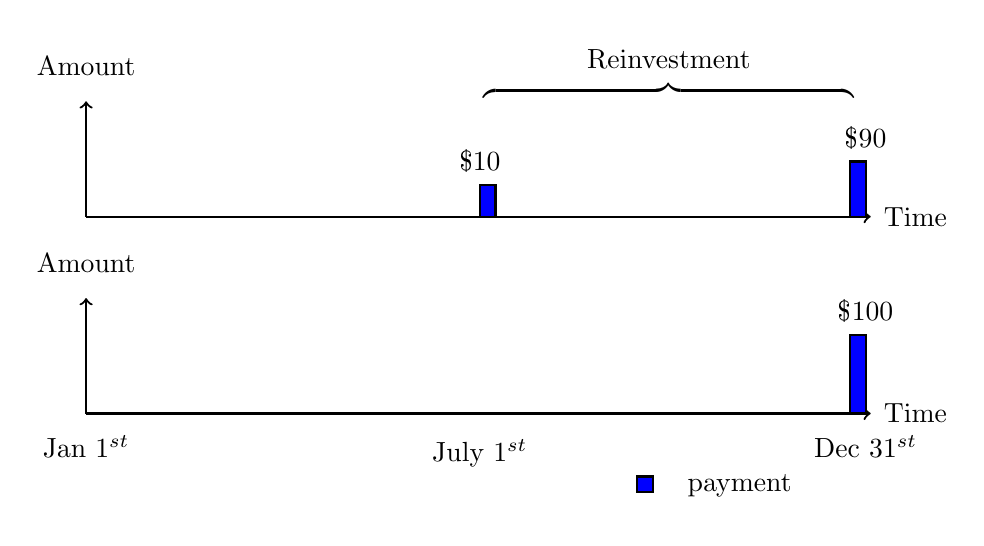
\begin{tikzpicture}[-,shorten >=1pt,auto,node distance=1.5cm,thick,minimum size=0.8cm,main node/.style={circle,draw=red,very thick}]
\tikzstyle{selected edge} = [draw,line width=6pt,-,blue!30]
\coordinate (belowstart) at (0,-1);

\coordinate (origo0) at (0,0);
\coordinate (xaxis0) at (10,0);
\coordinate (yaxis0) at (0,1.5);
\coordinate (face0s) at (9.9,0);
\coordinate (face0e) at (9.9,1.2);

\coordinate (origo1) at (0,2.5);
\coordinate (xaxis1) at (10,2.5);
\coordinate (yaxis1) at (0,4);
\coordinate (face1s) at (9.9,2.5);
\coordinate (face1e) at (9.9,3.3);

\coordinate (sixmpay1) at (5,2.5);
\coordinate (sixm1) at (5,2.80);

% Draw axes 0
\draw[->] (origo0) -- (xaxis0) node[right] {Time};
\draw[->] (origo0) -- (yaxis0) node[above] {Amount};

% Draw axes 1
\draw[->] (origo1) -- (xaxis1) node[right] {Time};
\draw[->] (origo1) -- (yaxis1) node[above] {Amount};
\draw[] (sixmpay1) -- (sixm1) node[above] {\$10};

% Draw reinvestment option
%\draw[dotted,draw=blue] (5.2,3.3) [bend left] (face1e);
\node[] at (7.4,4.1) {$\overbrace{\phantom{\hspace{4.7cm}}}$};
\node[] at (7.4,4.5) {Reinvestment};
\node[] at (5,-0.5) {July 1$^{\text{st}}$};

\filldraw[draw=black, fill=blue] (sixmpay1) rectangle node {} +(0.2,0.4);
\filldraw[draw=black, fill=blue] (9.7,2.5) rectangle node {} +(0.2,0.7);
\filldraw[draw=black, fill=blue] (9.7,0) rectangle node {} +(0.2,1);
%\filldraw[draw=black, fill=lightgray]  (10,1) rectangle node {} +(0.2,0.1);

% Legend
\filldraw[draw=black, fill=blue] (7,-1) rectangle node {} +(0.2,0.2);
\node at (8.3, -0.92) () {payment};
\node at (9.9,3.5) () {\$90};
\node at (9.9,1.3) () {\$100};

% "Legend"
\draw[] (origo0) -- (origo0) node[below] {Jan 1$^{\text{st}}$};
\draw[] (9.9,0) -- (9.9,0) node[below] {Dec 31$^{\text{st}}$};

\end{tikzpicture}
\caption{Two investment opportunities showing the time value of money.}
\label{fig:tvom}
\end{center}
\end{figure}

As investors want to maximize profits, it is quite intuitive to think that
the decision to invest directly depends on what alternatives are available.
Assuming resources are limited, it may quickly become difficult to asses which
option is opportune if the market offers multiple choices. As we saw above,
the discount factor is implicit given the rate, hence the reason for
\texttt{discountFactor} is part of the interface for interest rates.\\
Again we refer the reader to the documentation\cite{hqldoc} for examples of
how this is done in \hql.\\

Since we must consider all options to maximize our profits, we must somehow have an
overview of the interest rates currently offered in the market. This leads us onto the
next key element in pricing, namely the term structure of interest rates.

\section{Term Structure}\label{sec:ts}

A term structure can be viewed as a function f that given a tenor returns 
an interest rate. This rate reflects the expected return on an investment
over that period, meaning we may directly apply it to discount a cashflow
falling on the particular date implied by the tenor. It is also referred
to as a zero rate, as it is only usable to discount a independent cashflow
where there are no other intermittent payments over the tenor.

\begin{figure}[h!]
\begin{center}
\begin{tikzpicture}[-,shorten >=1pt,auto,node distance=1.5cm,thick,minimum size=0.8cm,main node/.style={circle,draw=red,very thick}]
\tikzstyle{selected edge} = [draw,line width=6pt,-,blue!30]
\coordinate (belowstart) at (0,-1);
\coordinate (xaxis) at (10,0);
\coordinate (origo) at (0,0);
\coordinate (yaxis) at (0,5);

% Draw axes
\draw[->] (origo) -- (xaxis) node[right] {Time to maturity};
\draw[->] (origo) -- (yaxis) node[above] {Annual rate};

% Flat TS
%\draw[thick,draw=blue] (0,1.5) -- (10,1.5);
% "Normal" TS
\draw[thick,draw=green] (0,0) parabola[bend at end] (10,5);
% Inverse TS
%\draw[thick,draw=red] (0,5) parabola[bend at end] (10,0.5);

\draw[dotted] (3,2.53) -- (3,0) node[below] {\text{ 3.5 years}};
\draw[dotted] (3,2.53) -- (0,2.53) node[left] {2.4\%};

% Legend
%\filldraw[draw=black, fill=blue] (5.2,-1) rectangle node {} +(0.2,0.2);
%\node at (6, -0.92) () {Flat};

%\filldraw[draw=black, fill=green] (0,-1) rectangle node {} +(0.2,0.2);
%\node at (1.55, -0.92) () {Logarithmic};

%\filldraw[draw=black, fill=red] (3,-1) rectangle node {} +(0.2,0.2);
%\node at (4.15, -0.92) () {Inverted};

\end{tikzpicture}
\caption{A example of a term structure.}
\label{fig:anc}
\end{center}
\end{figure}

A term structure of logarithmic shape as shown in \ref{fig:anc} characterizes a
"normal" market, where the return on an investment increases in some proportion
to the time you have tied up your funds\footnote{In reality, the shape depends on 
socio-economic factors such as growth or decline in the economy.}.\\

The term structure allows investors to observe at what price banks are
currently willing to loan money. We emphasize the time sensitivity of the term
structure, as external factors can cause sudden changes in the interest
rates and as a result the pricing of instruments (e.g. rate cuts by the
European Central Bank). By the time value of money it is possible to
appraise the value of an instrument (i.e. will the return on investment
be up to par with what a bank can offer?).\\

Turning to \hql, we need term structures to be able to price our cashflows.
Like interest rates, term structures come in different flavours and we 
have therefore also defined a data type to represent them:

\begin{hscode}
-- | A term structure is a yield curve constructed of
--- solely of zero rates.
data TermStructure = DiscreteTermStructure (Map Maturity Rate)
                   | AnalyticalTermStructure (Offset -> Rate)
                   | LinearInterpolatedTermStructure (Map Maturity Rate)
\end{hscode}

\ab{Do we need to import \texttt{Data.Map}?}

To better understand our data types we have shown them in figure \ref{fig:tstypes},
where we see that the \texttt{dfAt} is only defined at certain points in time for
a discrete term structure. Our \texttt{LinearInterpolatedTermStructure} is similar,
except it uses linear interpolation to estimate a term structure.
Finally, The analytical term structure is simply a function with domain $\mathcal{R}^+_0$
that maps an offset from valuation date to a zero interest rate over the given
period. This is necessary to represent a Nelson-Siegel generated function\cite{cmunk}.

In addition, we have defined the following functions to look up interest rates
or compute discount factors:

\begin{hscode}
type Factor = Double
-- | Returns the yield for a maturity
yieldAt :: TermStructure -> Maturity -> Maybe Rate
-- | Returns the discount factor at an offset
dfAt :: TermStructure -> Maturity -> Maybe Rate -- discount factor
-- | Returns the forward rate given two offsets
fwdRate :: TermStructure -> Maturity -> Maturity -> Maybe Factor
\end{hscode}

For instance, \texttt{yieldAt} function applied to the term structure in
figure \ref{fig:anc} with an offset of 3.5 years would produce $2.4\%$. We have
defined the following data types that are instances of the class above:

\begin{figure}[h!]
\begin{center}
\begin{tikzpicture}[-,shorten >=1pt,auto,node distance=1.5cm,thick,minimum size=0.8cm,main node/.style={circle,draw=red,very thick}]
\tikzstyle{selected edge} = [draw,line width=6pt,-,blue!30]

\coordinate (belowstart) at (0,-1);
\coordinate (xaxis) at (10,0);
\coordinate (origo) at (0,0);
\coordinate (yaxis) at (0,5);

% Discrete points
\coordinate (d0) at (1,1);
\coordinate (d1) at (2,2);
\coordinate (d2) at (3,3);
\coordinate (d3) at (4,3.5);
\coordinate (d4) at (5.6,4);
\coordinate (d5) at (7.5,4.5);
\coordinate (d6) at (9.2,5);

% Draw axes
\draw[->] (origo) -- (xaxis) node[right] {Offset from today (in years)};
\draw[->] (origo) -- (yaxis) node[above] {Interest rate};

% Analytical
\draw[thick,draw=purple] (0,0) parabola[bend at end] (10,5);

% Discrete
\node[minimum size=2pt,draw,circle,inner sep=1pt,fill] at (d0) {};
\node[minimum size=2pt,draw,circle,inner sep=1pt,fill] at (d1) {};
\node[minimum size=2pt,draw,circle,inner sep=1pt,fill] at (d2) {};
\node[minimum size=2pt,draw,circle,inner sep=1pt,fill] at (d3) {};
\node[minimum size=2pt,draw,circle,inner sep=1pt,fill] at (d4) {};
\node[minimum size=2pt,draw,circle,inner sep=1pt,fill] at (d5) {};
\node[minimum size=2pt,draw,circle,inner sep=1pt,fill] at (d6) {};

% Linear Interpolated
\draw[dotted,draw=blue] (origo) -- (d0);
\draw[dotted,draw=blue] (d0) -- (d1);
\draw[dotted,draw=blue] (d1) -- (d2);
\draw[dotted,draw=blue] (d2) -- (d3);
\draw[dotted,draw=blue] (d3) -- (d4);
\draw[dotted,draw=blue] (d4) -- (d5);
\draw[dotted,draw=blue] (d5) -- (d6);

% Today
\node at (0,-0.5) () {Today};
% Legend
\filldraw[draw=black, fill=blue] (5.2,-1.08) rectangle node {} +(0.2,0.2);
\node at (7, -1) () {Interpolated};

\filldraw[draw=black, fill=purple] (0,-1.08) rectangle node {} +(0.2,0.2);
\node at (1.55, -1) () {Analytical};

\filldraw[draw=black, fill=black] (3,-1.08) rectangle node {} +(0.2,0.2);
\node at (4.15, -1) () {Discrete};

\end{tikzpicture}
\caption{Visualization of our term structure types.}
\label{fig:tstypes}
\end{center}
\end{figure}

The reader should note that an interest rate with offset zero (that is, today) is
always zero, since nobody would be willing to lend you money for a single day.
Due to the inverse relation of interest rates and discount factors, the discount factor
today is always 1.

Moreover, the forward rate function, \texttt{fwdRate}, is used to obtain the 
implied future zero rates. There is no conceptual leap required to understand 
these, as they are simply interest rates in the future, hence the type 
signature requiring two offsets.\\
Notwithstanding, their usefulness is may not be evident. 
Imagine three points in time, $d_0$ - today - and two
offsets in the future $d_1$ and $d_2$. We are then tasked with finding out
what the interest rate between $d_1$ and $d_2$, $R_{12}$ would be. Despite not 
knowing whether the interest rate will increase or decrease we may specify 
this by introducing \emph{arbitrage}. In brief, no arbitrage is the
assumption it is not possible to buy and sell the same good and turn a
profit i.e. "free money". Given annual rates we can now claim the following:

\begin{equation}
\underbrace{(1+R_{02})^2}_{observable} = \underbrace{(1+R_{01})}_{observable}(1 + R_{12})
\end{equation}

where $R_{xy}$ denotes the rate between two points in time $x$ and $y$. We
can now solve for $R_{12}$ to obtain the forward rate. Forward rates therefore
allow us to make statements about future interest rates as a result of the
prevailing interest rates.

% TODO more

\section{Instruments}\label{sec:instruments}

Now that we have cemented the basic theory of interest rates, discounting
and term structures we turn to their application in financial instruments.

We have defined an \texttt{Instrument} class to represent the high-level
functionality that all financial instruments must share:

%%% Explain the Instrument class %%%
\begin{hscode}
-- | Instrument is a high-level class for financial instruments
class Instrument i where
  -- | Is the instrument expired?
  expired :: i -> IO Bool
  -- | Underlying model required for pricing
  type PricingEngine :: *
  -- | Returns the present value of the instrument
  pv :: i -> PricingEngine -> IO Cash
\end{hscode}

We require an associated type to represent a pricing engine since we
cannot price all instruments in a similar fashion.\\
Due to the high-level nature of this class, very few methods qualify.
It is interesting to note that \hql defines the
exact same two functions as Quantlib's \texttt{Instrument}
class\cite{implql}. Also, Quantlib has an equivalent \texttt{PricingEngine}
class to cater for the need of different pricing methods for different
products.\\

\begin{figure}[!h]
\centering
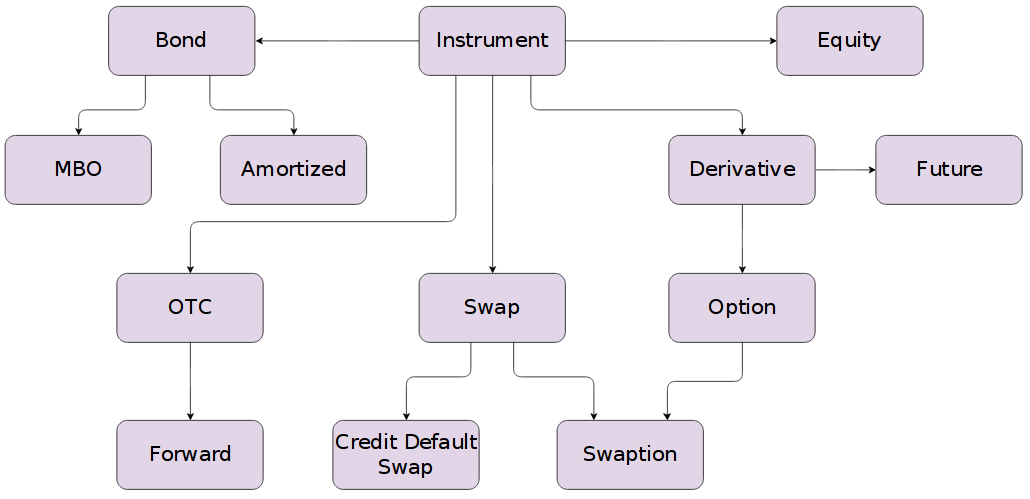
\includegraphics[scale=.3]{images/classhier.png}
\caption{Type class architecture.}
\label{fig:classhier}
\end{figure}

In the coming sections we shall delve into the specific instruments and
describe their implementations. We refer the reader to figure \ref{fig:classhier}
for and overview of the classes we have defined. The arrows denote type class
constraints e.g. a \texttt{Bond} must be an instance of \texttt{Instrument}.

\section{Fixed Income}\label{sec:fi}

In this section we will go through how we have modelled the subset of products 
in the \emph{fixed income} category, of which a product called bonds are 
the bread and butter. In brief, a bond is a financial security that promises
the bond holder a stream of future payments. These play a huge role in the 
financial markets are are typically only offered by governments or large 
financial institutions.\\
We will present our \texttt{FixedIncome} module by means of a running example
of a bond. A \emph{serial} is an example of a bond that equates to a typical 
Danish house loan. The cash flow of the holder of a 5 year serial with annual 
repayments is depicted in figure \ref{fig:serialcf}.\\

\begin{figure}[!h]
\begin{center}
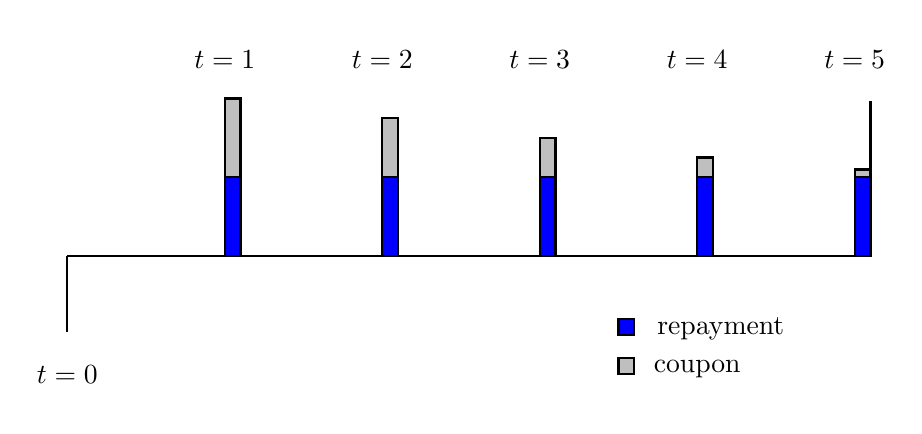
\begin{tikzpicture}[-,shorten >=1pt,auto,node distance=1.5cm,thick,minimum size=0.8cm,main node/.style={circle,draw=red,very thick}]
\tikzstyle{selected edge} = [draw,line width=6pt,-,blue!30]

\coordinate (belowstart) at (0,-1);
\coordinate (start) at (0,0);
\coordinate (stop) at (10.2,0);
\coordinate (abovestop) at (10.2,2);
\draw (start) -- (stop);
\draw (start) -- (belowstart);
\draw (stop) -- (abovestop);

\node at (0, -1.5) () {$t=0$};

\filldraw[draw=black, fill=blue] (2,0) rectangle node {} +(0.2,1);
\filldraw[draw=black, fill=lightgray]  (2,1) rectangle node {} +(0.2,1);
\node at (2, 2.5) () {$t=1$};

\filldraw[draw=black, fill=blue] (4,0) rectangle node {} +(0.2,1);
\filldraw[draw=black, fill=lightgray]  (4,1) rectangle node {} +(0.2,0.75);
\node at (4, 2.5) () {$t=2$};

\filldraw[draw=black, fill=blue] (6,0) rectangle node {} +(0.2,1);
\filldraw[draw=black, fill=lightgray]  (6,1) rectangle node {} +(0.2,0.5);
\node at (6, 2.5) () {$t=3$};

\filldraw[draw=black, fill=blue] (8,0) rectangle node {} +(0.2,1);
\filldraw[draw=black, fill=lightgray]  (8,1) rectangle node {} +(0.2,0.25);
\node at (8, 2.5) () {$t=4$};

\filldraw[draw=black, fill=blue] (10,0) rectangle node {} +(0.2,1);
\filldraw[draw=black, fill=lightgray]  (10,1) rectangle node {} +(0.2,0.1);
\node at (10, 2.5) () {$t=5$};

% Legend
\filldraw[draw=black, fill=blue] (7,-1) rectangle node {} +(0.2,0.2);
\node at (8.3, -0.92) () {repayment};

\filldraw[draw=black, fill=lightgray] (7,-1.5) rectangle node {} +(0.2,0.2);
\node at (8, -1.44) () {coupon};

\end{tikzpicture}
\caption{Cashflow of a serial.}
\label{fig:serialcf}
\end{center}
\end{figure}

We observe that the bond issuer makes fixed size deposits to the counterpart to 
repay the loan. Since there is no such thing as a free lunch, so-called coupon 
payments are made in addition to compensate for having its funds tied up. These
payments are simply the bond's interest rate applied to the face value of the
bond, and are decreasing as a result of the repayment amortization\cite{hqldoc}.\\

In addition to the serial, we present the most basic bond imaginable, the zero 
coupon bond or simply \emph{zero}. It is exactly that - a bond with a specified 
tenor and interest rate that pays a fixed amount at maturity.\\

We have designed a class to encapsulate the functionality of bonds:

%%% Explain the Bond class %%%
\begin{hscode}
type Payment = (Date,Cash) -- A payment is cash on some date
type Payments = [Payment]
-- | Bond class specifies common denominator for all bond types 
class Instrument b => Bond b where
  -- | Returns dirty price on a given date
  dirty :: TermStructure ts => b -> ts -> Date -> Cash
  -- | Principal (or face value) of a bond
  principal    :: b -> Cash
  -- | A list of Payments indicating remaining cashflow
  outstanding  :: b -> Payments
  -- | Returns a list of Payments representing the cashflow
  -- over the bond over its lifetime
  cashflow     :: b -> Payments
  -- | Returns the coupon part of the cashflow
  coupons      :: b -> Payments
  -- | Returns the dates at which cashflow is exchanged
  paymentDates :: b -> [Date]
\end{hscode}

The \texttt{cashflow} function generates a list of payments exactly as shown
in figure \ref{fig:serialcf} while \texttt{coupons} generates only the coupon
payments. We define a function \texttt{dirty}, which is used by the \texttt{pv}
function to return the price of a bond at a specific bond. "Dirty" means that
the price does not take into account the time value of money if the bond is
sold between two coupon payments. A "clean" price also exists that accounts
for the accrued interest between two payments.\\

A serial is an example of an \emph{amortized} bond, meaning that the writer
of a serial (the person who initially lended the money) receives repayments over
the lifetime of a bond. As these loan-based bonds come in multiple flavours
we have therefore created an \texttt{Amortized} class:

\begin{hscode}
-- | Class declaration for amortized bonds
class Bond a => Amortized a where
  repayments :: a -> Payments
\end{hscode}

allowing users to retrieve a list of payments representing the coupon payment
subtracted from the cashflow. \texttt{repayments} now generate the blue repayment part of the cashflow
we observe in figure \ref{fig:serialcf}.\\

Returning to our serial example, we have defined a data type for fixed coupon
amortized bonds using a Haskell generalized algebraic data type (GADT):

\begin{hscode}
data FixedAmortizedBond where 
  Annuity :: { asett :: Date,
               amatu :: Date,
               aface :: Cash,
               arate :: Double,
               astms :: Settlements,
               adcc  :: (DayCount d) => d,
               aroll :: RollConvention } -> FixedAmortizedBond
  Serial :: {  asett :: Date,
               amatu :: Date,
               aface :: Cash,
               arate :: Double,
               astms :: Settlements,
               adcc  :: (DayCount d) => d,
               aroll :: RollConvention } -> FixedAmortizedBond
\end{hscode}

where the fields are explained in table \ref{tab:fields}.\\

\begin{center}  
\begin{longtable}{l|l|l}
Field & Meaning & Usage\\\hline
\texttt{asett} & Settlement date & Start date for interpolation\\
\texttt{amatu} & Maturity date & End date for interpolation\\
\texttt{aface} & Face Value & Used to compute repayment and coupons\\
\texttt{astms} & Settlements per Year & Used to generate payment dates\\
\texttt{adcc} & Daycount convention & Used in discounting\\
\texttt{aroll} & Roll convention & Resolves illegal payment dates (e.g. weekends)\\
\caption{\texttt{FixedAmortizedBond} fields}
\end{longtable}
\label{tab:fields}
\end{center}

Note that although the \texttt{Annuity} loan has the same fields as our serial,
we need a separate constructor for it as the cashflow generation is completely
different for this bond type\cite{hqldoc}. In addition to the zero and amortized
bonds, \hql also features various other bond types\cite{hqldoc}.

%%% Haskell %%%
A central tenet of our architecture is that we keep the backend
as simple as possible and keep the interface detailed and 
self-explanatory. This way we keep the mathematical formulas as transparent
and clean as possible while the interface remains user-friendly.\\

The backend for pricing bonds exploits the fact that all instances must define
the \texttt{cashflow} function. As we saw in section \ref{sec:discounting},
pricing a cashflow is simply multiplication by a discount factor. This means
that pricing a bond $b$ can be formulated as follows:

\begin{equation}
PV_b = \sum_{k=0}^n df_k cf_k
\end{equation}

where $cf_k$ and $df_k$ denote a cashflow or discount factor at time $k$,
respectively. As a result, the backend for bond pricing is implemented as:

\begin{hscode}
pv = sum $ zipWith (*) cashflowList discountFactors
\end{hscode}

\section{Options, Futures and other Derivatives}

In this section we briefly describe how our architecture caters to other
financial products in addition to the fixed income instruments we have seen.\\

In figure \ref{fig:classhier} we defined the inheritance relations that
exist in terms of financial products and how we are to model them using 
Haskell's class system. \hql currently implements the toolbox required
for the implementation of the resulting products. The only constraint on
new additions to \hql is the \texttt{Instrument} class which all products
must be an instance. This means that the challenge lies the the fact
that we must define an appropriate \texttt{PricingEngine} type for each
class of products.\\

A \emph{call option} is a contract that gives the holder the right to purchase
(or \emph{exercise} a good or service (this is called the \emph{underlying}) 
at a specific price (the \emph{strike}). What pricing engine is appropriate 
for such a contract; does it depend on the underlying?
In fixed income we saw that the term structure of interest rates qualified,
but this is not the case for options.

Instead, we may want to use a Black-Scholes model for European
options or a binomial model for American\footnote{The distinction
between American and European has nothing to do with geography. European
options may only be exercised at maturity, while American ones can be
exercised at any time.} options\cite{HULL}.

While it is possible to price European-style options using a closed-form 
solution, we must apply simulation methods to price the American counterpart.
The computations required should be reflected by the declaration of
\texttt{PricingEngine}.
